%!TEX root = ../../../adrien_gomar_phd.tex

\subsection{Introduction}
\label{sub:ca_introduction}

The contra-rotating open rotor architecture is a classical engine
turbomachinery whose fan is not within a nacelle. As explain
above, this help increasing the mass-flow of the primary flow
which leads to a higher propulsive efficiency.
Two main architectures are retained. One based on a gearbox, the second
being build around a statorless low-pressure turbine.
\begin{figure}[htb]
  \centering
  \subfigure[Geared design]{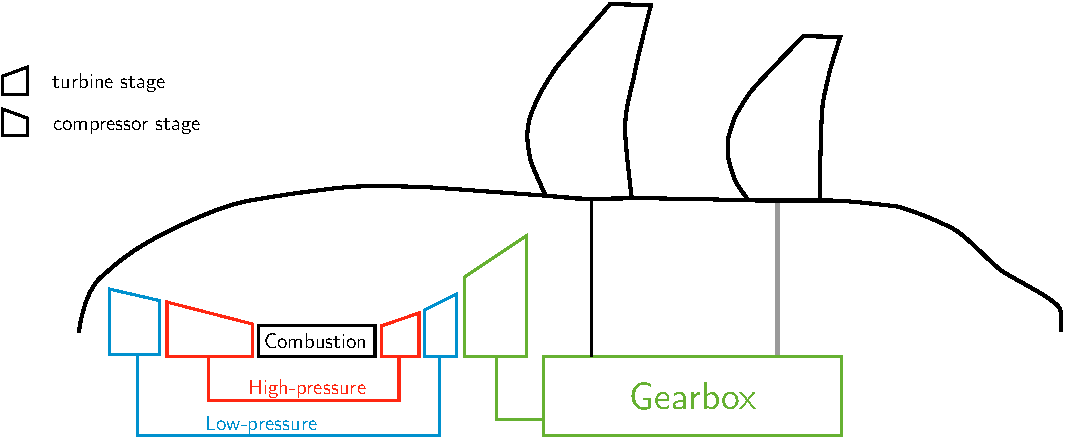
\includegraphics[width=.4\textwidth]{geared_cror.pdf}}
  \subfigure[Statorless low-pressure turbine design]{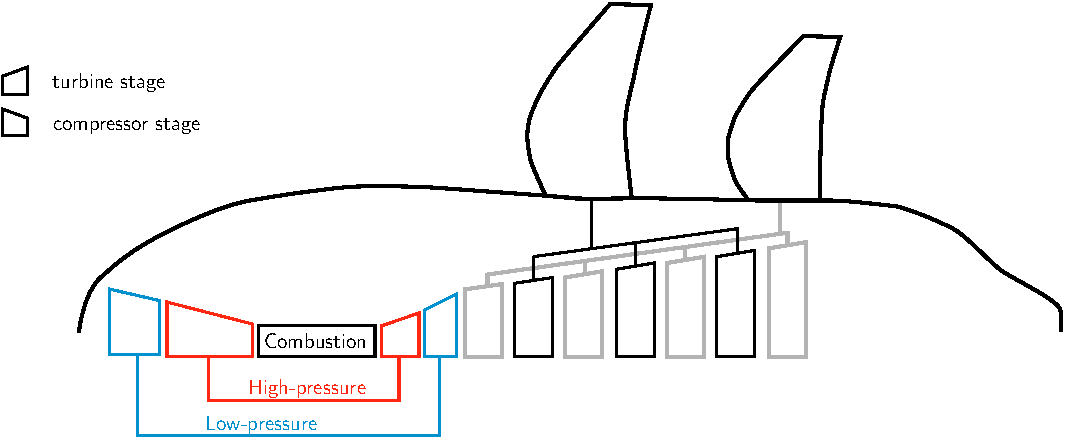
\includegraphics[width=.4\textwidth]{stator_less_cror.pdf}}
  \caption{Contra-rotating open rotor architectures.}
  \label{fig:ca_cror_designs}
\end{figure}

The basic idea behind the CROR concept is that a propeller has a 
better propulsive efficiency than a turbofan. The problem is that
a residual tangential velocity is present behind a propeller.
In fact, applying the velocity triangle to a propeller configuration
as shown in Fig.~\ref{fig:ca_velocity_triangle_propeller}, one can
observe that the outlet velocity (noted $V^{out}_x$) is not axial
leading a tangential velocity $\Delta V_{\theta}$. This tangential forms
the swirl observe behind a propeller. First, this is a lost energy and
second, it produces a torque that has an impact on the flight dynamics
of the airplane. To alleviate this effect, one can use two propellers
that are counter-rotating as for instance the TP$400$ propellers
in the Airbus-A$400$M military airplane.

To recover this lost energy, a second contra-rotating rotor is used.
\begin{figure}[htb]
  \centering
  \subfigure[propeller]{
  	\label{fig:ca_velocity_triangle_propeller}
  	\includegraphics*[scale=0.4]{velocity_triangle_propeller.pdf}}
  \subfigure[contra-rotating open rotor]{
  	\label{fig:ca_velocity_triangle_cror}
  	\includegraphics*[scale=0.4]{velocity_triangle_cror.pdf}}
  \caption{Velocity triangle applied to a propeller and a 
  contra-rotating open rotor configuration.}
\end{figure}
Figure~\ref{fig:ca_velocity_triangle_cror} shows the application
of the velocity triangle to a CROR configuration. The swirl
energy that was lost in the propeller is now used to 
produce more thrust. Thus, the CROR has a better propulsive
efficiency than the propeller.

\subsection{General flow physics} % (fold)
\label{sub:general_flow_physics}

% subsection general_flow_physics (end)

\subsection{Similarity coefficients}
\label{sub:ca_similarity_coeff}

To allow the comparison and the assessment of several
propeller configurations, four similarity coefficients are used:
the advance ratio $J$, the traction coefficient $C_t$, 
the power coefficient $C_p$ and the efficiency $\eta$.
These are defined as:
\begin{alignat}{4}
    J &= \frac{V_0}{n D} \label{eq:advance_ratio}, \\
    C_t &= \frac{F_x}{\frac{1}{2} n ^ 2  D ^ 4}, \\
    C_p &= \frac{M_x \Omega_{rad.s-1}}{\frac{1}{2} n ^ 3 D ^ 5}, \\
    \eta &= J \frac{C_t}{C_p},
\end{alignat}
where $V_0$ is the free-stream velocity, 
$n$ the rotation frequency ($n = \Omega_{rad.s-1} / 2 \pi$) with 
$\Omega_{rad.s-1}$ being the rotation speed of the propeller, $D$ the diameter
of the propeller, $F_x$ and $M_x$ the axial force and torque respectively.

In the case of a CROR configuration, two propellers are actually considered.
